\section{Theorie}
% Es sollen die wichtigsten theoretischen Formeln und Zusammenh�nge einmal ausf�hrlich erkl�rt werden
In diesem Abschnitt sollen die wichtigsten theoretischen Grundlagen f�r den Versuch dargestellt werden.
\subsection{Reflexion und Brechung elektromagnetischer Wellen an der ebenen Trennfl�che zweier Dielektrika}
An dem Schaubild in Abbildung \ref{fig:Brechung} soll die vorliegende Situation der Brechung einer elektromagnetischen Welle an einer Grenzfl�che dargestellt werden.
\begin{figure}[H]
\centering
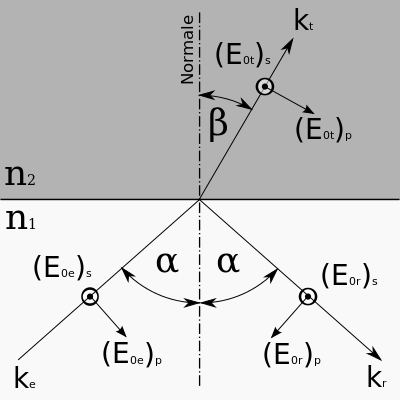
\includegraphics[clip = true, scale = 0.75]{ReflexionAmplitudenverhalten.png}
\caption{Die Einfallsebene wird von \textbf{k} und \textbf{n} aufgespannt, sodass die Polarisation des elektrischen Feldes relativ zur Einfallsebene angegeben werden kann. Quelle: \cite{wiki_fresnel}}
\label{fig:Brechung}
\end{figure}
Die Brechungsindizes sind dabei definiert als $ n_1 = \sqrt{\frac{\mu_1\epsilon_1}{\mu_0\epsilon_0}} $ und $ n_2 = \sqrt{\frac{\mu_2\epsilon_2}{\mu_0\epsilon_0}}$, mit den Permittivit�ten $\epsilon$ und Permeabilit�ten $\mu$ der beiden Medien. Dabei bezeichnet $\text{E}_{\text{0e}}$ das E-Feld der einfallenden Welle, $\text{E}_{\text{0r}}$ das E-Feld der reflektierten Welle und $\text{E}_{\text{0t}}$ das E-Feld der transmittierten Welle.
\subsection{Snelliussches Brechungsgesetz}
Das Snelliussche Brechungsgesetz beschreibt die Richtungs�nderung der Ausbreitungsrichtung ebener elektromagnetischer Wellen bei der Brechung an einer ebene Trennfl�che zweier Dielektrika. Da die r�umliche und zeitliche �nderung aller Felder in der Brechungsebene (z = 0) die gleiche sein muss, m�ssen auch die Phasenfaktoren der drei Wellen (Abb. \ref{fig:Brechung}) unabh�ngig von der Art der Grenzbedingung in der Brechungsebene (z = 0) �bereinstimmen (vgl. \cite{Jackson}). Daraus folgt das Snelliussche Brechungsgesetz:
\begin{align}
(\textbf{k}_{\textbf{e}}\cdot \textbf{x})_{z=0} = (\textbf{k}_{\textbf{t}}\cdot \textbf{x})_{z=0} = (\textbf{k}_{\textbf{r}}\cdot \textbf{x})_{z=0}
\label{eqn:Snel_Brech}
\end{align}
Aus $c |\textbf{k}| = \sqrt{\mu_r \epsilon_r}\cdot\omega = \text{n}\omega$ ergibt sich die �blichere Darstellung des Brechungsgesetzes durch Gleichung \ref{eqn_Snel}.
\begin{align}
\text{n}_1\sin(\alpha) = \text{n}_2\sin(\beta)
\label{eqn_Snel}
\end{align}
\subsection{Fresnelsche Formeln}
Mit den Fresnelschen Formeln kann die Intensit�t, Phasen�nderung und die Polarisation des gebrochenen Lichtstrahls berechnet werden. Sie basieren auf den Maxwellgleichungen und den Stetigkeitsbedingungen der Felder an der Trennfl�che. In diesem Versuch ist die relative Permeabilit�t $\mu_r$ im wesentlichen 1, da mit sichtbarem Licht gearbeitet wird. F�r diesen Spezialfall lauten die Reflektionskoeffizienten, die sich aus den Fresnelschen Formeln ergeben:
\begin{align}
r_s = \frac{\text{n}_1\cos(\alpha)-\text{n}_2\cos(\beta)}{\text{n}_1\cos(\alpha)+\text{n}_2\cos(\beta)}
\label{eqn:Fres_r_s}
\\
r_p = \frac{\text{n}_2\cos(\alpha)-\text{n}_1\cos(\beta)}{\text{n}_2\cos(\alpha)+\text{n}_1\cos(\beta)} 
\label{eqn:Fres_r_p}
\end{align}
Mit dem Snelliusschen Brechungsgesetz k�nnen diese Formeln ebenso unabh�ngig von $\beta$ dargestellt werden (vgl. \cite{Jackson}).